\documentclass{article}
\usepackage{tikz}
\usetikzlibrary{shapes,arrows}


\begin{document}

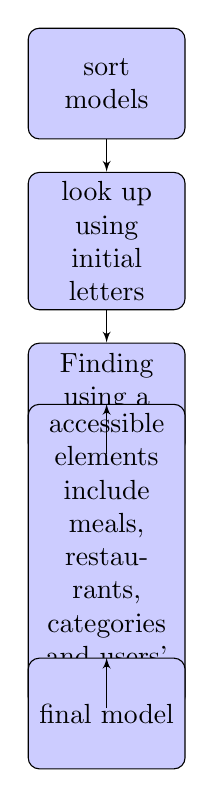
\begin{tikzpicture}[node distance = 2cm, auto]

    % Define block styles
    \tikzstyle{block} = [rectangle, draw, fill=blue!20,
        text width=5em, text centered, rounded corners, minimum height=4em]
    \tikzstyle{line} = [draw, -latex']

    % Place nodes
    \node [block] (init) {sort models};
    \node [block, below of=init] (identify) {look up using initial letters};
    \node [block, below of=identify] (evaluate) {Finding using a binary tree};
    \node [block, below of=evaluate] (tune) {accessible elements include meals, restaurants, categories and users' cards};
    \node [block, below of=tune] (final) {final model};

    % Draw edges
    \path [line] (init) -- (identify);
    \path [line] (identify) -- (evaluate);
    \path [line] (evaluate) -- (tune);
    \path [line] (tune) -- (final);

\end{tikzpicture}

\end{document}